\chapter{Experiments and results}

\label{kap:experiments} % id kapitoly pre prikaz ref

For all experiments we used data from \textit{NA12878 Oxford Nanopore Human Reference Datasets} \cite{data}. 
This dataset provides a lot of basecalled reads in fast5 format aligned to reference DNA. 

For our experiments, we used $40$ blocks of $1000$ bases with corresponding parts of squiggles provided by 
bachelor thesis by Jakub Havelka \cite{kubo}.

To analyze the quality of our consensus signal, we used basecaller \textit{ONT Albacore Sequencing Pipeline Software (version 2.2.4)}.
At first, we basecalled each aligned squiggle and a consensus signal. 
Then for each DNA sequence produced, we calculated alignment
score by aligning it to the corresponding part of the reference sequence 
using Needleman-Wunsch algorithm described in \ref{nwalg}.

\section{Results}
We tested multiple methods of multiple alignments and signal reconstruction on all 40 datasets.
Each graph shows alignment score of squiggles (blue) and consensus signal (red).
Each column in graphs represents one dataset.

Figure \ref{fig:final3} shows results of consensus signal produced by \textit{aligning to sequence} and 
signal reconstruction with \textit{simple average} after each alignment. We can see that consensus signal produced in some cases slightly better results than each squiggle but in most cases resulted in average quality.

\begin{figure}
  \centering
  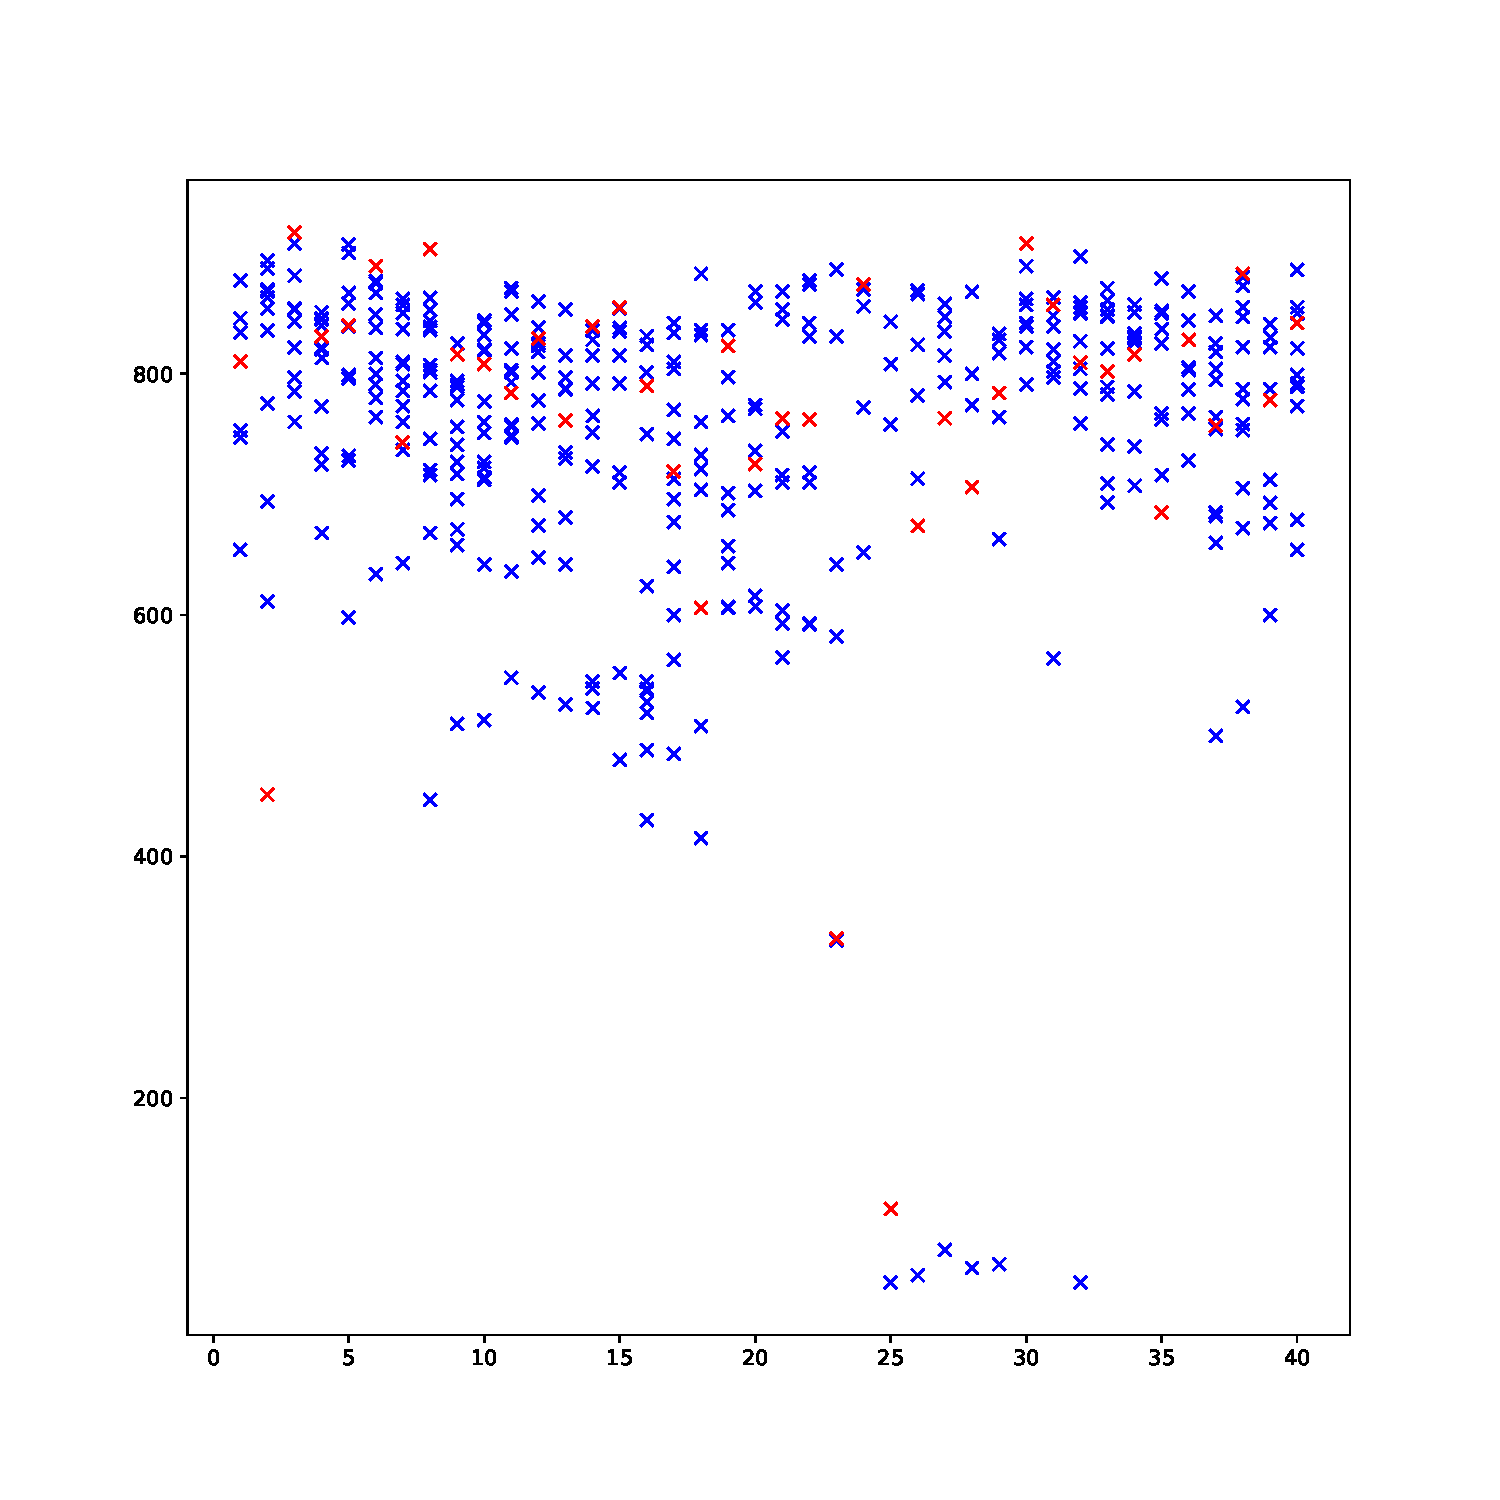
\includegraphics[width=1.0\textwidth]{images/final3}
  \caption{\textit{Aligning to sequence} and signal reconstruction with \textit{simple average} after each alignment.}
  \label{fig:final3}
\end{figure}

Figure \ref{fig:final2} shows results of consensus signal produced by \textit{aligning to sequence} and
final signal reconstruction by \textit{average with length adjustment}. This Approach produced best results with better alignment
score in more than $25\%$ of datasets.

\begin{figure}
  \centering
  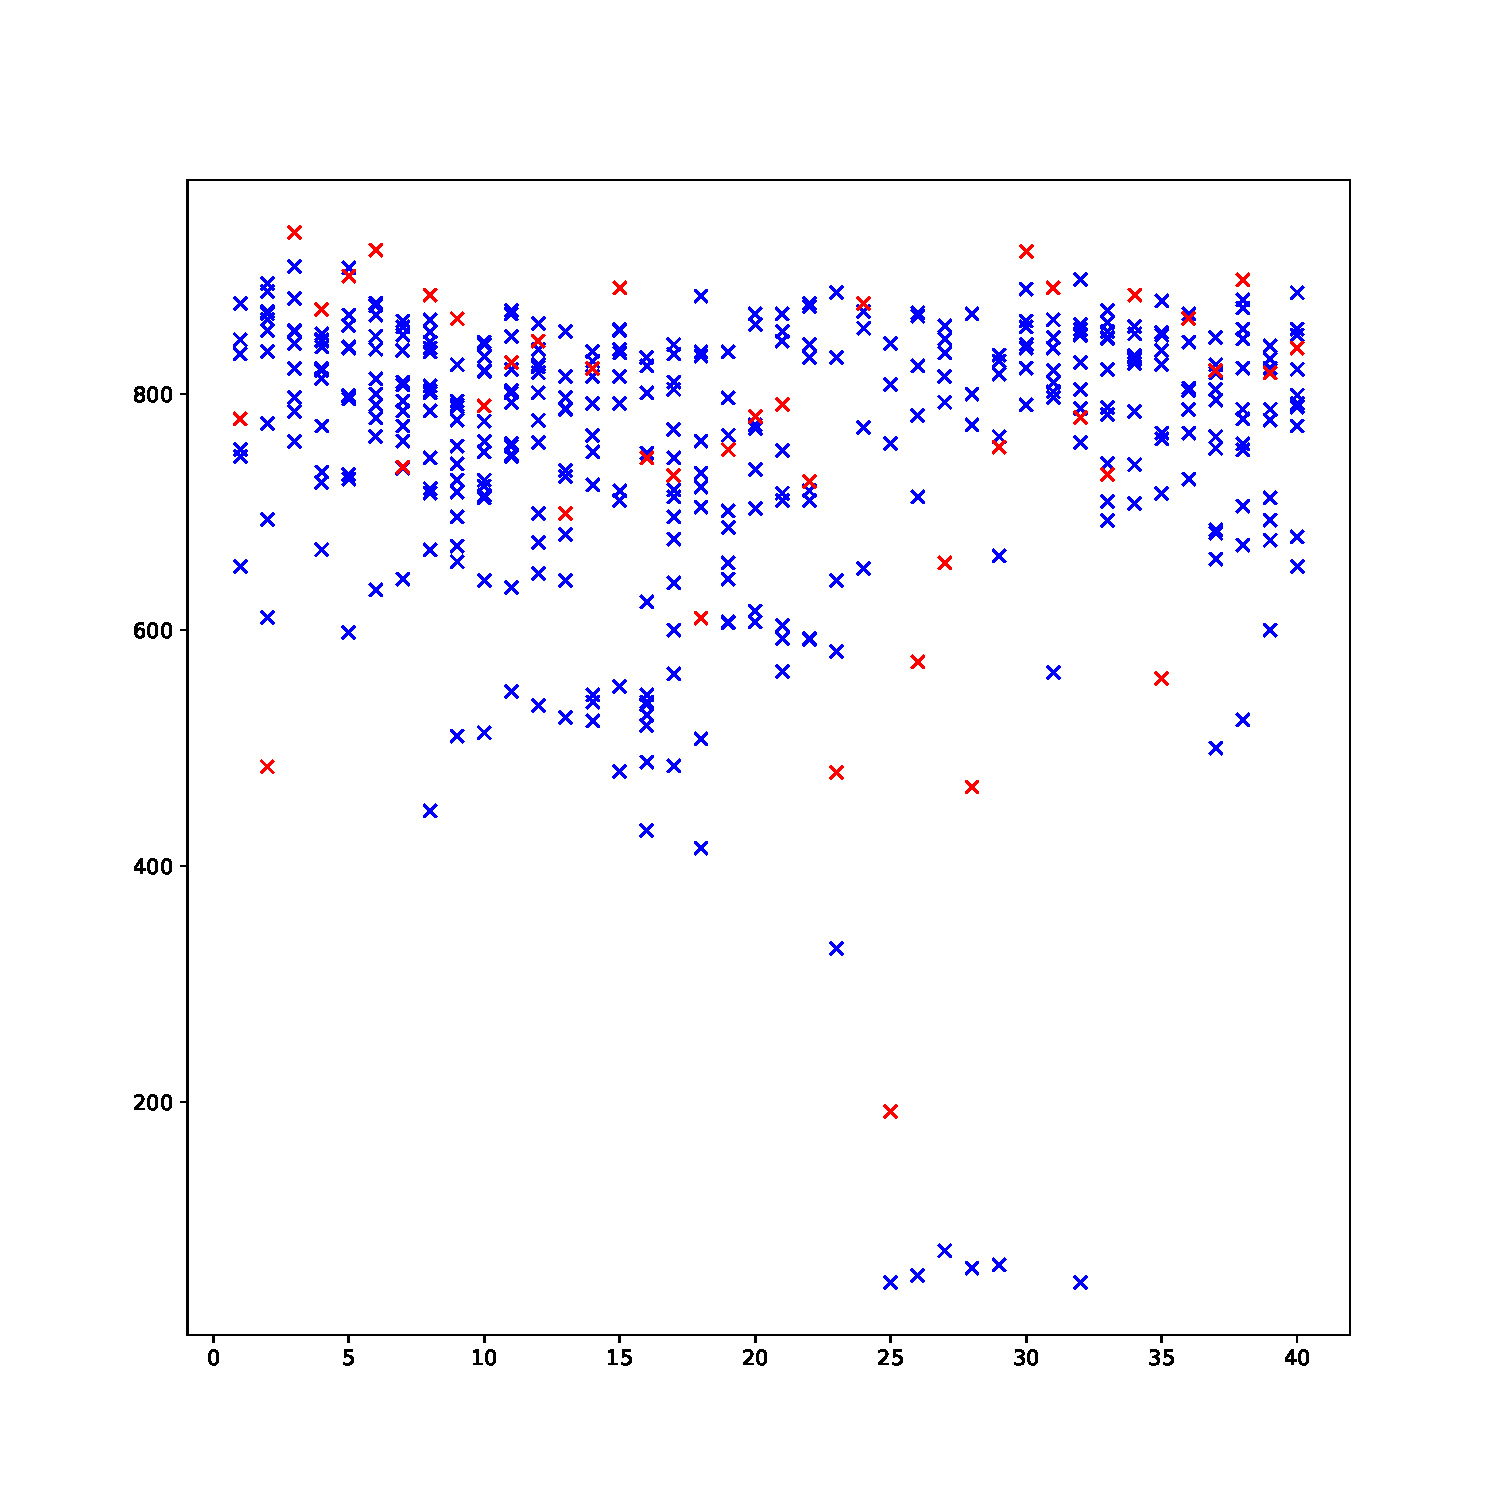
\includegraphics[width=1.0\textwidth]{images/final2}
  \caption{\textit{Aligning to sequence} and final signal reconstruction by \textit{average with length adjustment}.}
  \label{fig:final2}
\end{figure}


Figure \ref{fig:final6} shows results of consensus signal produced by \textit{aligning to sequence} and
signal reconstruction by \textit{average with length adjustment} after each alignment. This approach led to bad results
in all cases. 

\begin{figure}
  \centering
  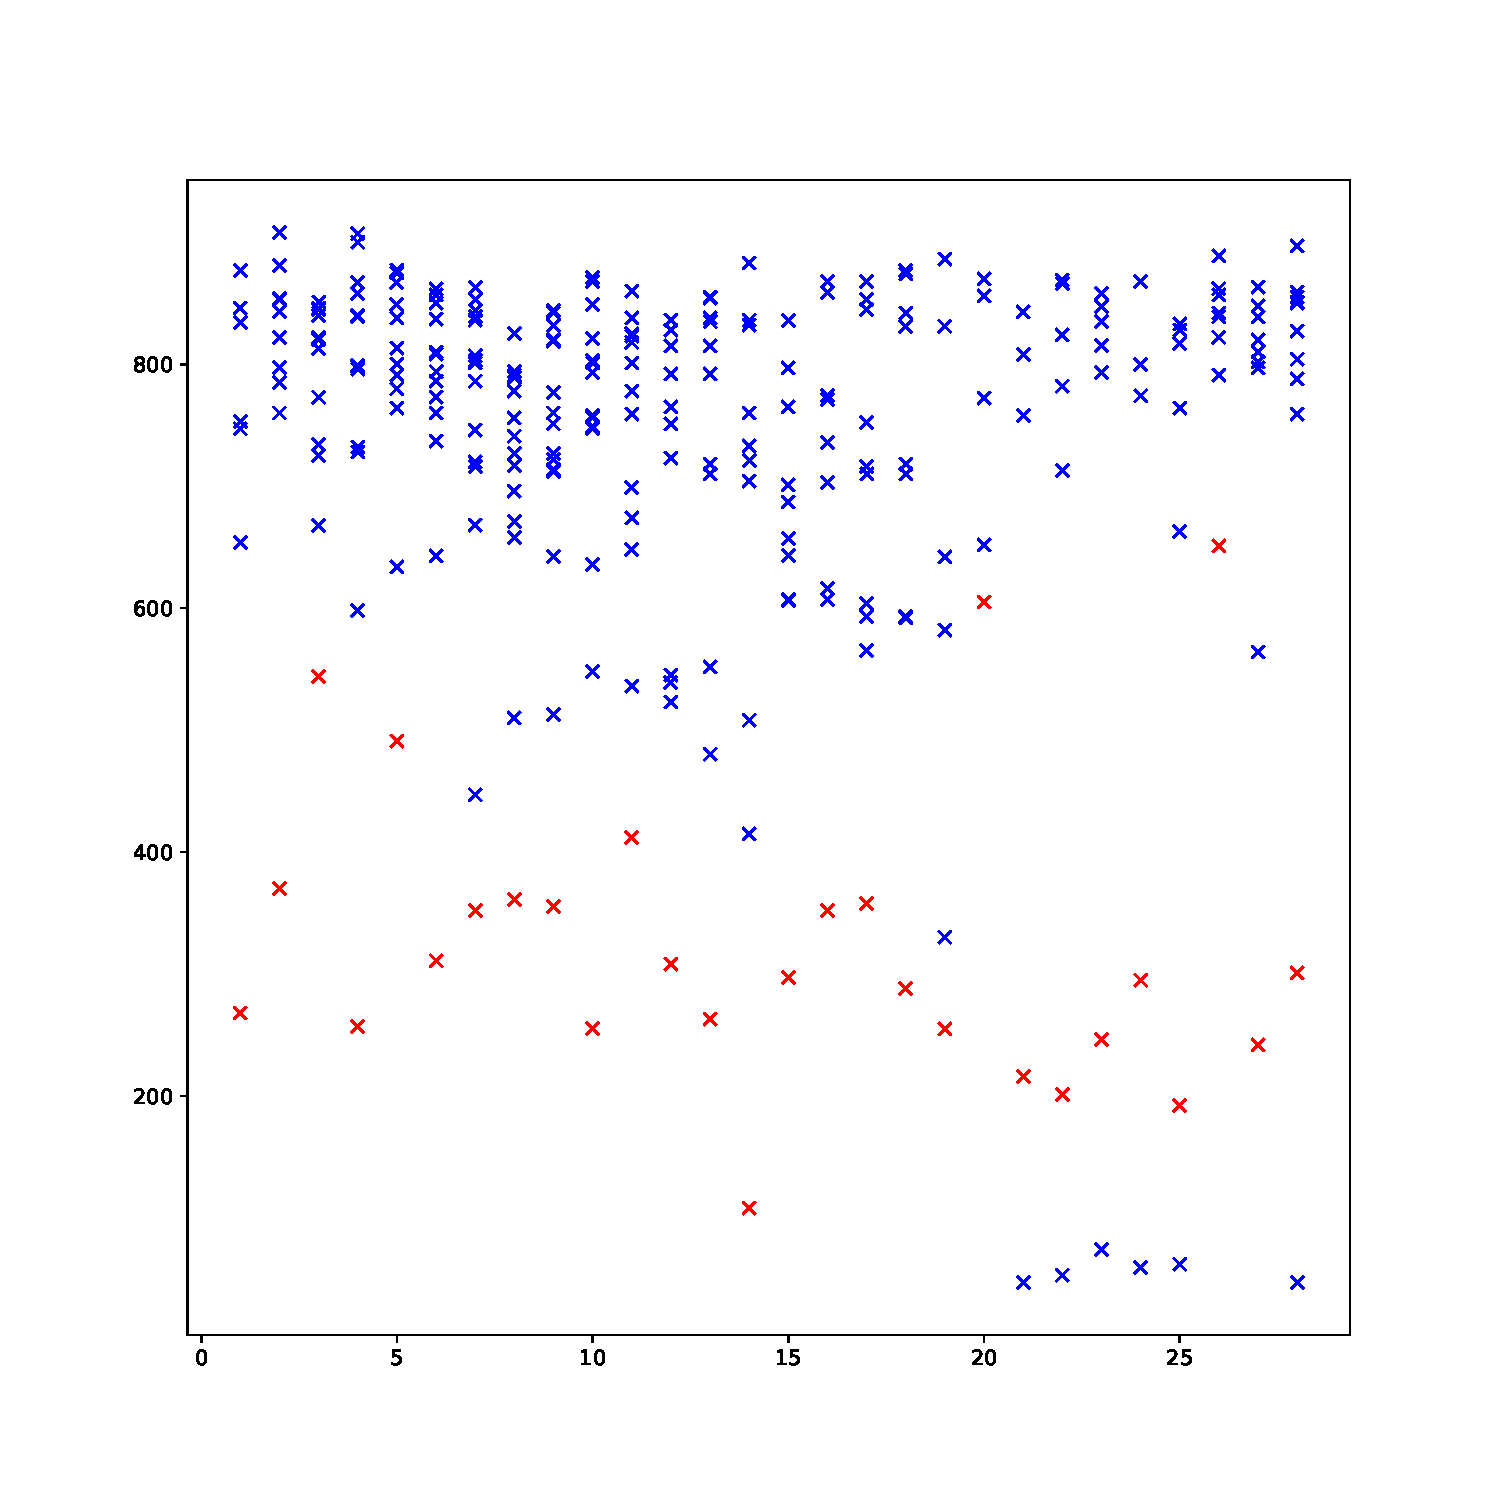
\includegraphics[width=1.0\textwidth]{images/final6}
  \caption{\textit{Aligning to sequence} and signal reconstruction by \textit{average with length adjustment} after each alignment.}
  \label{fig:final6}
\end{figure}

Figure \ref{fig:final4} shows results of consensus signal produced by \textit{complete alignment} and 
signal reconstruction by \textit{simple average}. In this case, in some datasets resulting signal did not even pass 
quality filter of basecaller.

\begin{figure}
  \centering
  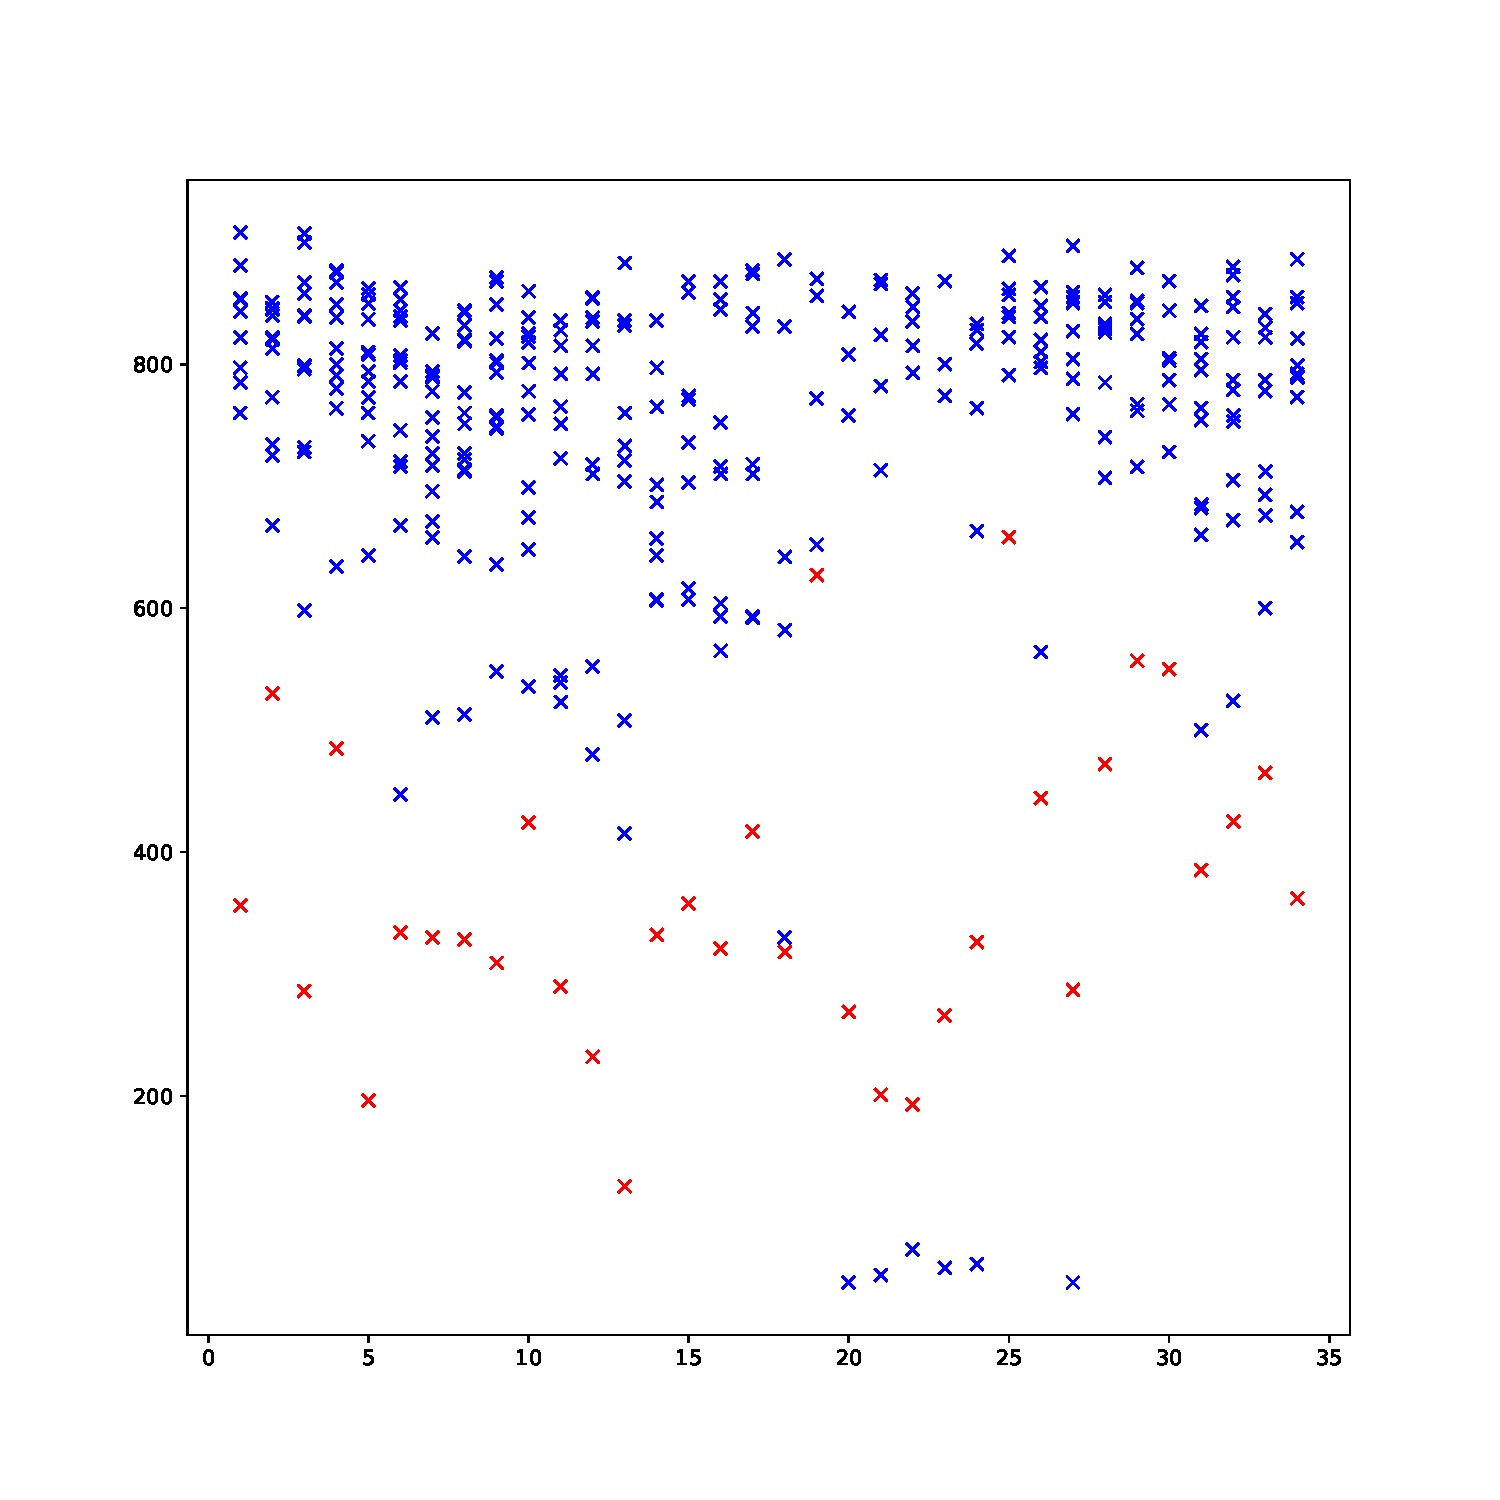
\includegraphics[width=1.0\textwidth]{images/final4}
  \caption{\textit{Complete alignment} and signal reconstruction by \textit{simple average}.}
  \label{fig:final4}
\end{figure}

Figure \ref{fig:final5} shows results of consensus signal produced by \textit{complete alignment} and 
final signal reconstruction by realigning all squiggles to it by \textit{aligning to sequence} and
final signal reconstruction by \textit{average with length adjustment}. 

\begin{figure}
  \centering
  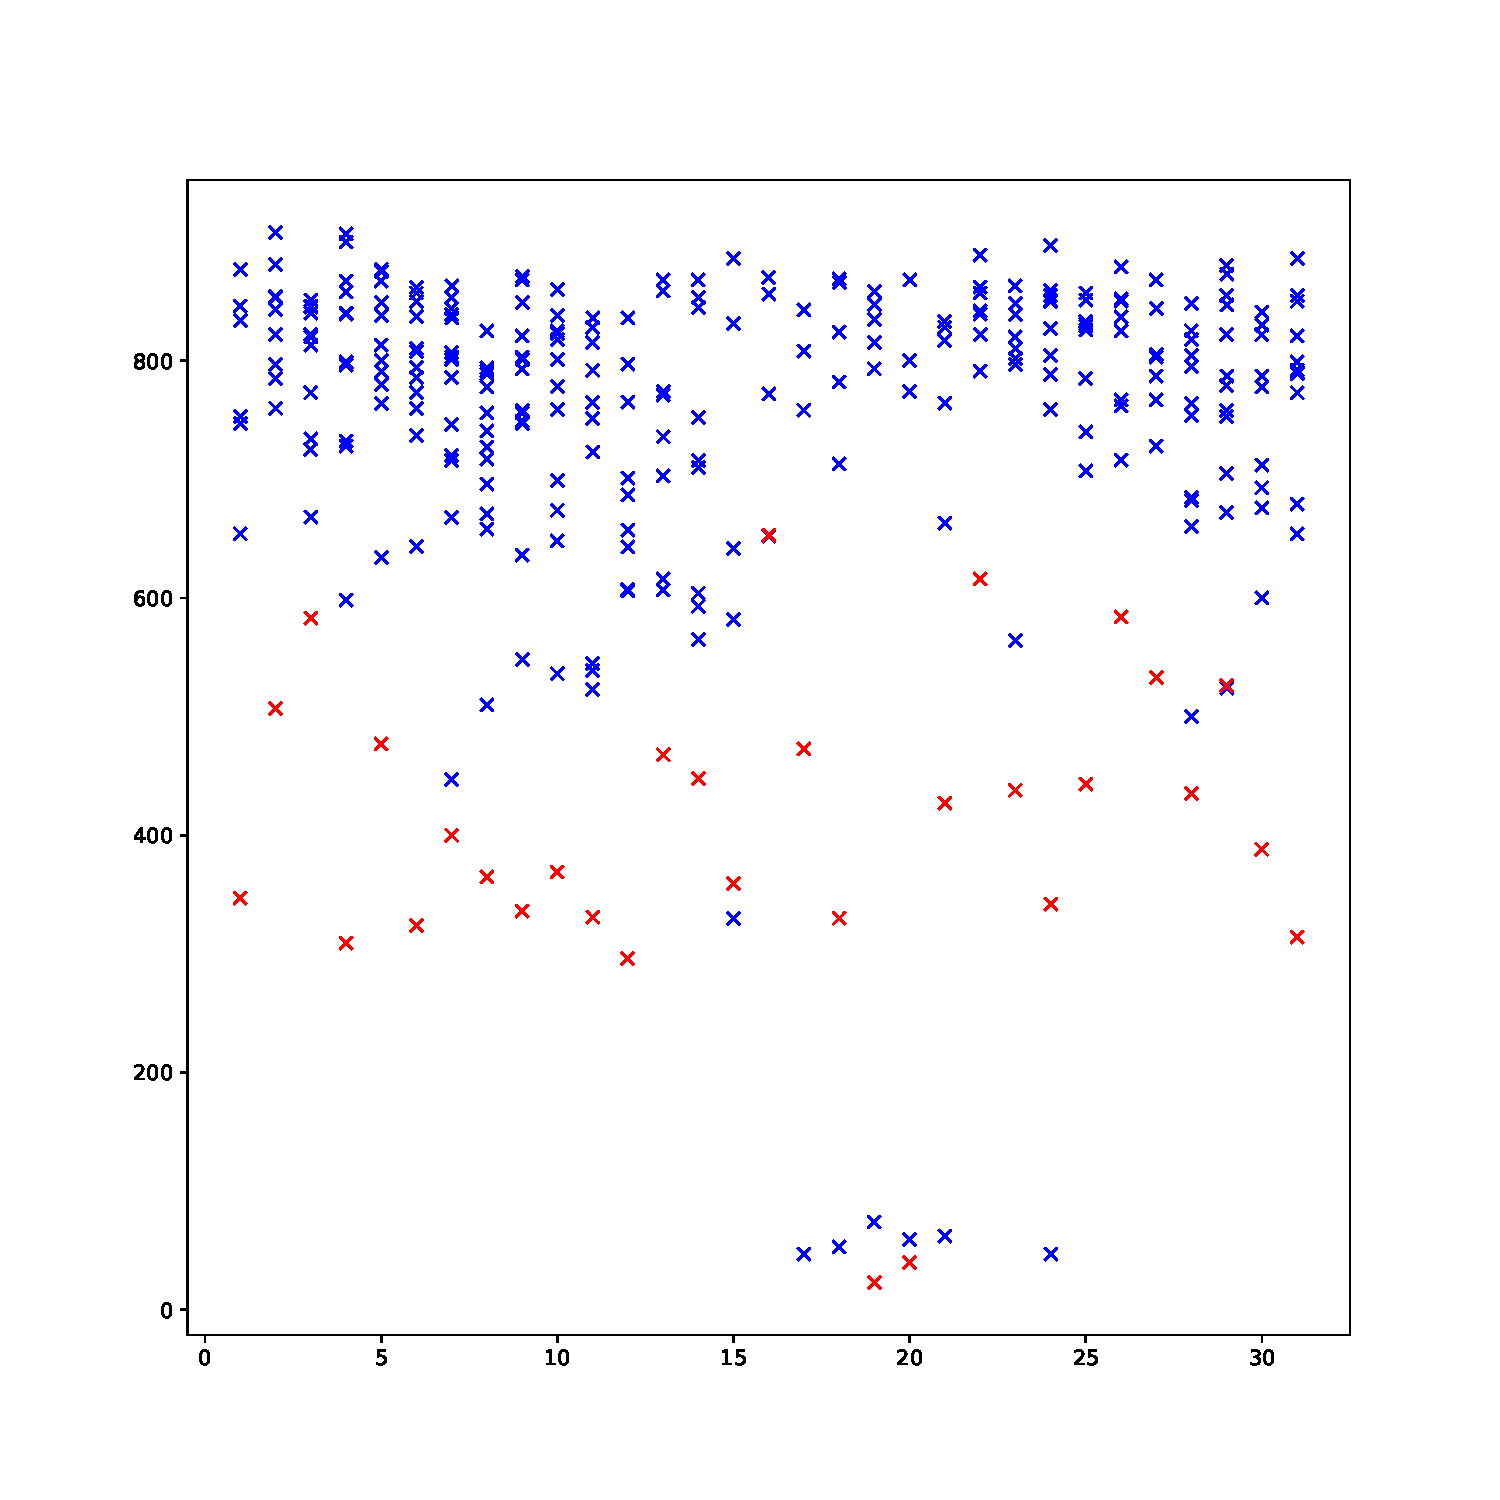
\includegraphics[width=1.0\textwidth]{images/final5}
  \caption{\textit{Complete alignment} and final signal reconstruction by realigning all squiggles to it.}
  \label{fig:final5}
\end{figure}